%%%%%%   TIPO DE DOCUMENTO: ArtIculo   %%%%%%
\documentclass[letterpaper,11pt]{article}

%%%%%%%  ESPECIFICACION DE PAQUETES   %%%%%
\usepackage[spanish]{babel} %Lenguaje: Espanol
\usepackage{graphicx} %Manejo de imagenes
\usepackage[utf8]{inputenc}
\usepackage{amsmath,amssymb,amsfonts}
\usepackage{graphicx} % Imagenes 
\usepackage{cite} 
\usepackage{hhline}
\usepackage{multicol}
\usepackage{longtable}
\usepackage{amssymb}
\usepackage{t1enc}
\usepackage{amsmath}
\usepackage{color}
\usepackage{pdfpages}
\usepackage{subcaption}
%\usepackage{hyperref}
\usepackage{listings}
\usepackage{float}
\usepackage{url}
\usepackage{textcomp}
\usepackage{musixtex}

%%%%%%%    INICIO DEL CUERPO DEL DOCUMENTO    %%%%%%%
\begin{document}

  %%%%%%%   INCLUYE PORTADA   %%%%%%%
  
\begin{center}
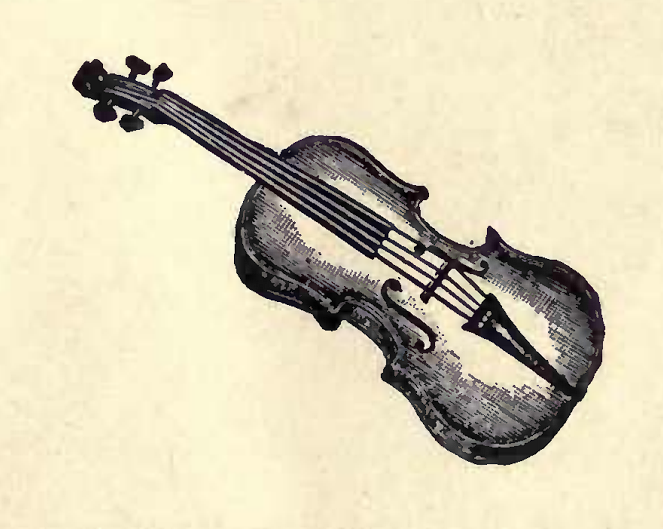
\includegraphics[width=0.5\textwidth]{../img/violin.png}
\end{center}

\begin{center}
\textbf{LOWELL, INDIANA.\\
Alfred Ha Miller}

\textbf{Copyright 1906,\\
Por Frederick Castle, M. D.\\
H. H. RAGON \& SON, Impresores,\\
Lowell, Indiana.\\
1906.}
\end{center}

\begin{center}
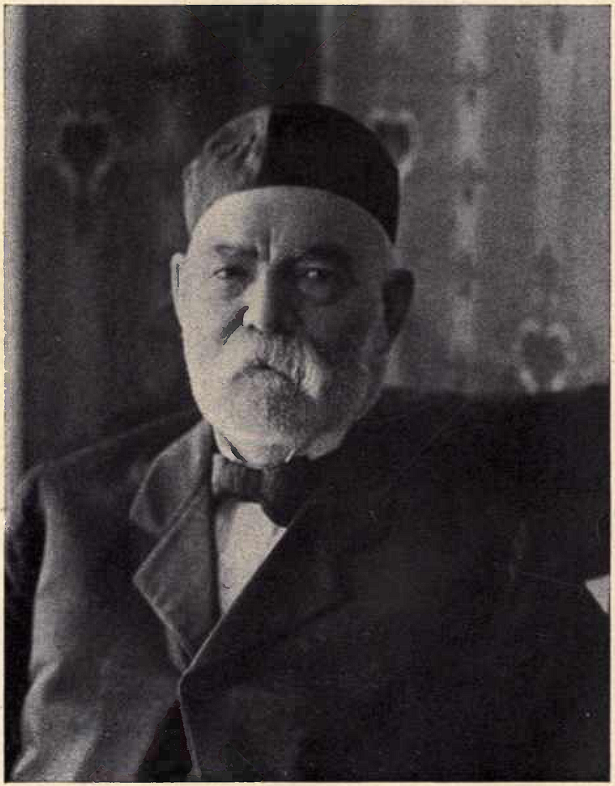
\includegraphics[width=1\textwidth]{../img/foto.png}
\par\smallskip
    \textbf{DR. FREDERICK CASTLE. }
\end{center}

  %%%%%%%   INCLUYE SECCIONES   %%%%%%%
  \section{T\'itulo de la secci\'on 1}

Este es el contenido agregado de la secci\'on 1.

$criptoan\acute{a}lisis$ %SecciOn 1

  %\bibliographystyle{abbrv} %{plain}
  %\bibliography{bibliografia}
\end{document}
